\documentclass[preview]{standalone}

\usepackage{amsmath}
\usepackage{amssymb}
\usepackage{stellar}
\usepackage{bettelini}

\hypersetup{
    colorlinks=true,
    linkcolor=black,
    urlcolor=blue,
    pdftitle={Biologia},
    pdfpagemode=FullScreen,
}

\begin{document}

\title{Biologia}
\id{biologia-biomi}
\genpage

\begin{snippetdefinition}{bioma-definizione}{Bioma}
    Un \textit{bioma} è una vasta regione del mondo caratterizzata da forme dominanti
    di piante e clima, che interagiscono producendo una comunità biotica distinta e unica.
\end{snippetdefinition}

\begin{snippet}{biome-illustration-1}
    \begin{center}
    \begin{figure}[th]
        \centering
        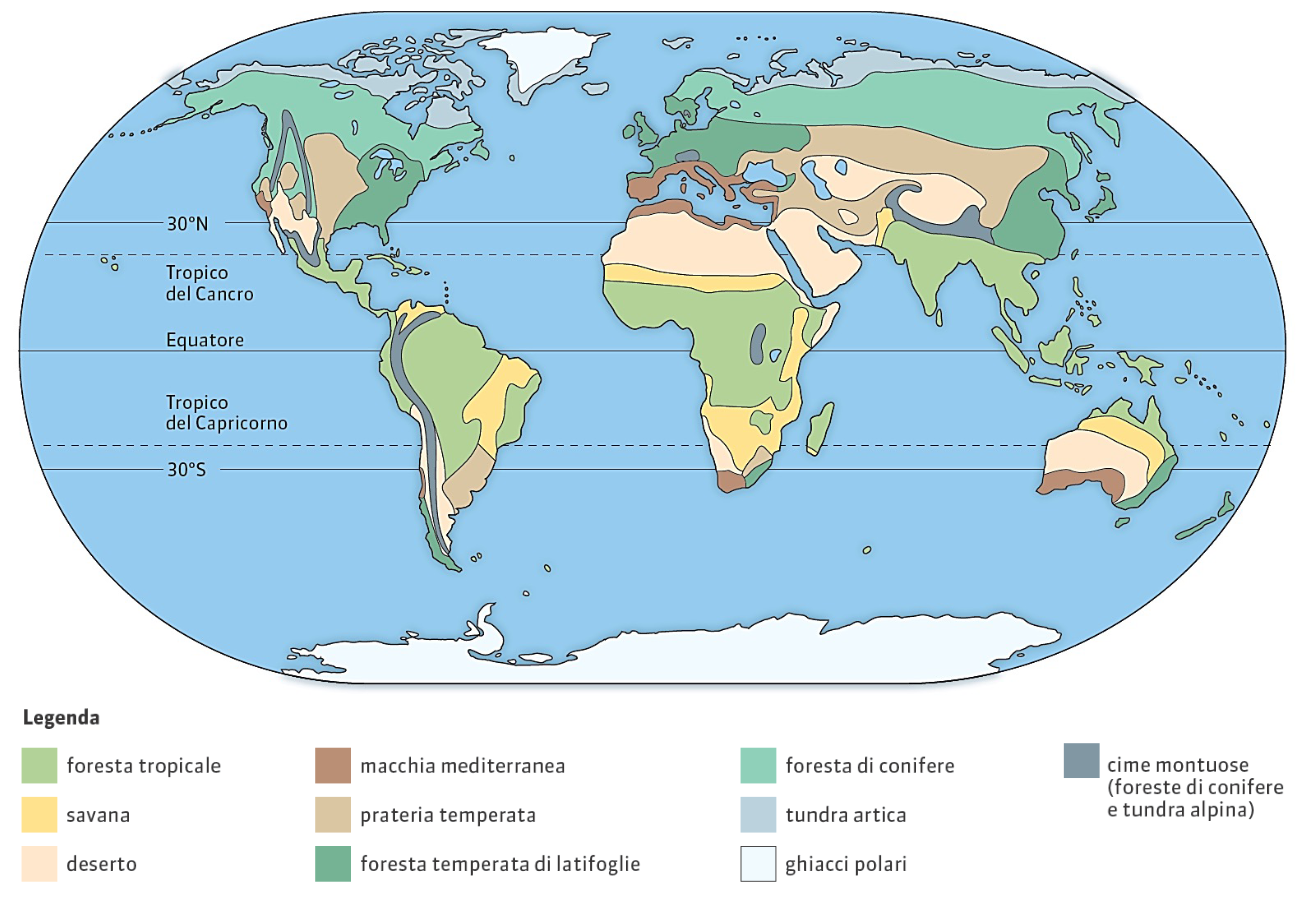
\includegraphics[width=\textwidth]{./resources/biomi1.png}
    \end{figure}
    \end{center}
\end{snippet}

\plain{La foresta di conifere e la tundra artica sono presenti solo in un emisfero.}

\begin{snippet}{biome-illustration-2}
    \begin{center}
    \begin{figure}[th]
        \centering
        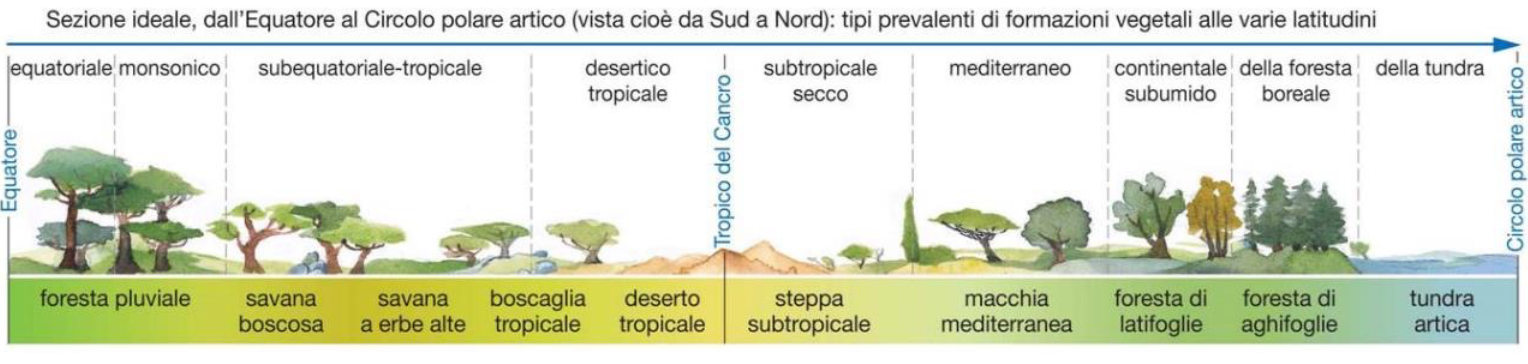
\includegraphics[width=\textwidth]{./resources/biomi2.png}
    \end{figure}
    \end{center}
\end{snippet}

\end{document}